\documentclass[11pt,a4paper,oneside]{article}
\usepackage[latin1]{inputenc}
\usepackage{amsmath}
\usepackage{amsfonts}
\usepackage{amssymb}
\usepackage{graphicx}
\usepackage{color}
\usepackage {tikz}
\usepackage{fancyvrb}
\usepackage{multicol}
\usepackage{caption}
\usepackage{subfig}
\usetikzlibrary {er}
\usepackage[left=2.00cm, right=2.00cm, top=1.00cm]{geometry}
\graphicspath{{./}}
\fvset{tabsize=4}

\begin{document}
	\title{DS 294 - Data Analysis and Visualization - Assignment 1}
	\author{Shriram R. \\ M Tech (CDS) \\ 06-02-01-10-51-18-1-15763}
	\maketitle	
	
	\section{Gephi}
	Gephi [1] is an open source visualization software for graphs and networks. This software comes under the Information Visualization tier. It allows the user to interact, manipulate the structures, shapes and colors of graph visualization. It enables exploratory data analysis and is a complementary tool for statistics. Gephi supports many kind of graphs (directed, undirected, mixed) and associated formats. The following sections provide a summary of its features along with screenshots of the tool.
	
	\subsection{Features}
	
    \textbf{Layout} - Gephi implements advanced layout algorithms designed for both efficiency and quality. The algorithms are Force-based and optimized for graph readability. The layout can be changed dynamically during runtime as well.\\	
	\textbf{Metrics} - Gephi provides a statistics and metrics framework for some of the common network analysis. These include Betweenness Centrality, Closeness, Diameter, Clustering Coefficient, PageRank, Community Detection, Shortest Path etc.\\	
	\textbf{Filtering} - Gephi has capabilities to filter nodes and edges based on network structure and data. It provides an interactive user interface to filter the network in real-time. It supports complex filter queries and saving of query results.\\	
	\textbf{Data Edition} -	Gephi comes with its own Data laboratory with an Excel-like interface to edit data columns, search and transform data. It also supports batch edit mode, customized column merge etc.\\	
	\textbf{Cartography} - Gephi allows ranking and partitioning of data for meaningful network representation. Users can customize colors, size or labels of the network. It has a vectorial preview module and can save presets and export visualization into PDF, SVG and PNG format.\\	
	\textbf{Temporal Analysis} - Gephi provides full support for dynamic graph analysis. It allows the users to visualize how a network or graph evolve over time by manipulating the embedded timeline. It can import temporal graph and can run metrics over time such as clustering coefficient and supports graph streaming.\\	
	\textbf{Performance} - Gephi has a fast visualization engine based on OpenGL and supports graphs upto 100,000 nodes and 1,000,000 edges. Users can iterate through several edits and the changes are rendered in real-time.\\	
	\textbf{Graph Generation} -	Gephi comes with a graph generation tool that can generate random graphs, dynamic graphs and multigraphs. Users can specify the number of nodes and wiring probability and the tool can quickly generate a graph as per the specification.\\	
	\textbf{Extensibility} - There are numerous community developed plugins to extend the functionalities. There is a in-built Plugins Center which can automatically pull the list of plugins available from the Gephi PLugin portal nad performs all kind of software updates.\\
	
	\subsection{Screenshots}	
	The above screenshots are taken using the Les Miserables: coappearance weighted network of characters dataset [2] consisting of 77 vertices and 254 edges.
			
	\begin{figure}%
		\centering
		\subfloat[Nodes colored by degree and Force Layout]{{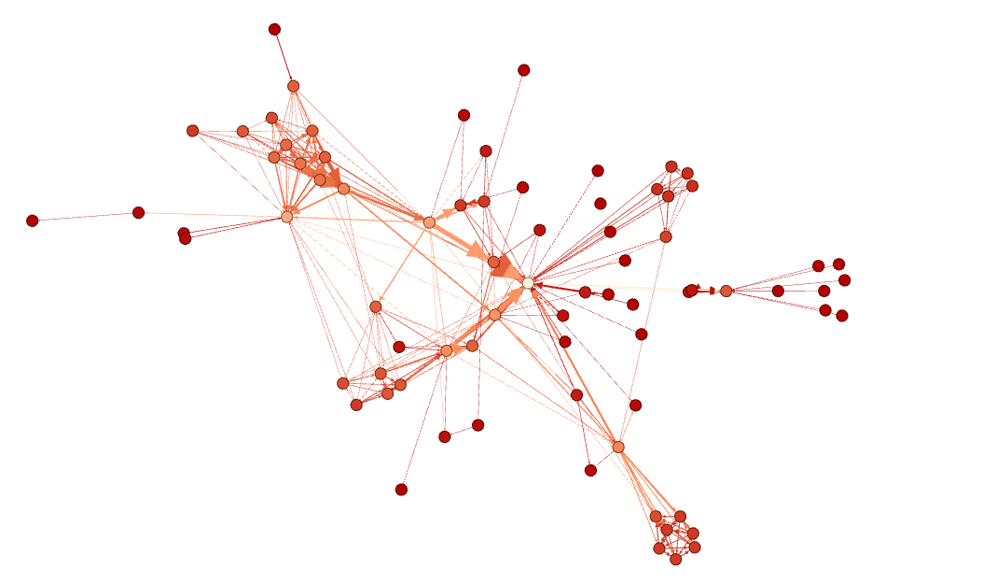
\includegraphics[width=7.5cm]{1.png} }}%
		\qquad
		\subfloat[Community Detection and Partitioning]{{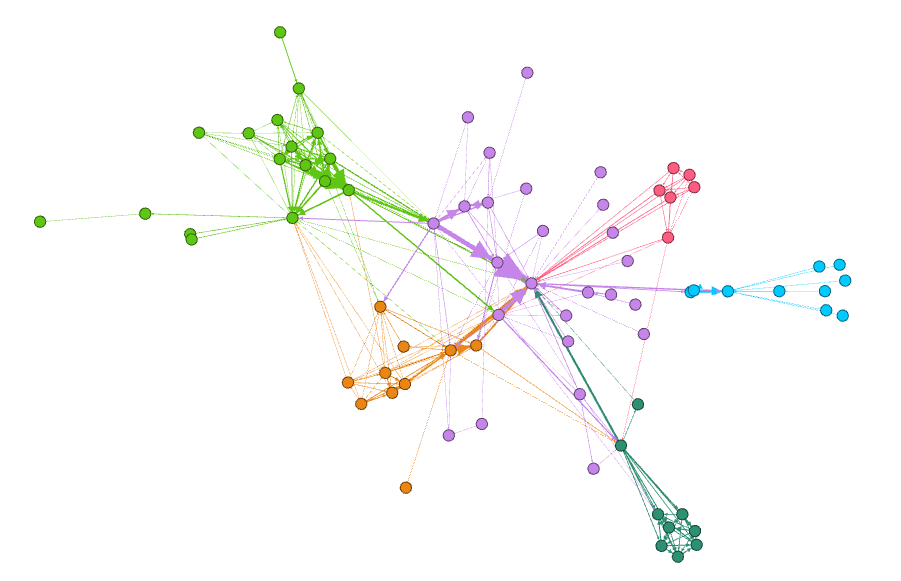
\includegraphics[width=7.5cm]{3.png} }}%
		\qquad
		\subfloat[Eigenvector Centrality Distribution]{{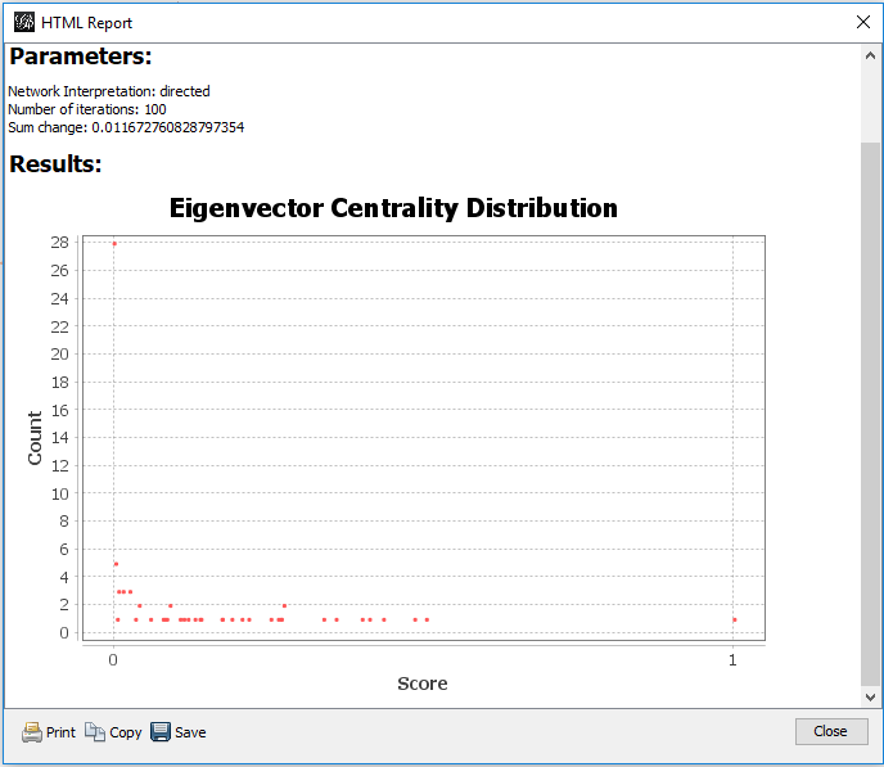
\includegraphics[width=7.5cm]{2.png} }}%
		\qquad
		\subfloat[Fruchterman Reingold Layout]{{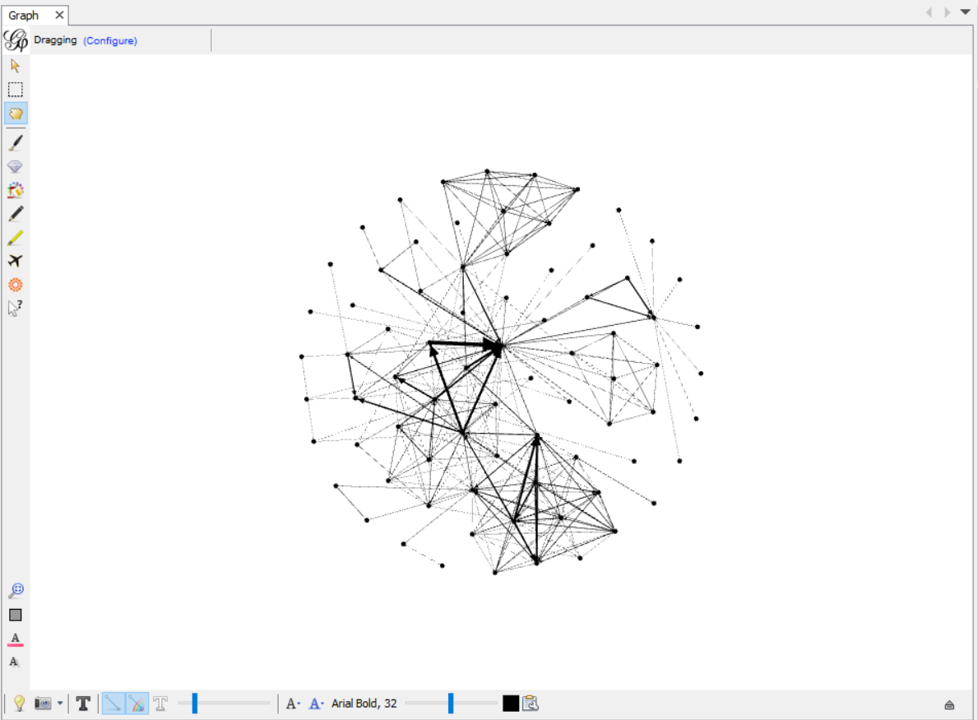
\includegraphics[width=7.5cm]{6.png} }}%
		\qquad
		\subfloat[Data Edit Mode]{{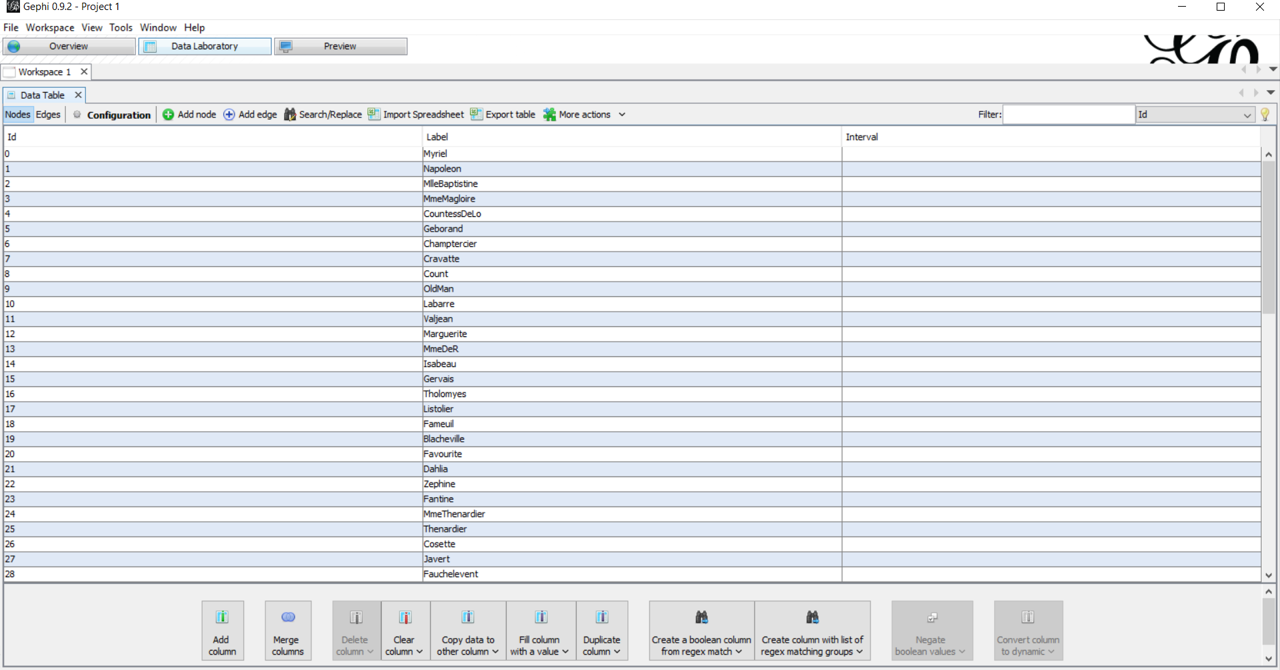
\includegraphics[width=7.5cm]{5.png} }}%
	    \qquad
	    \subfloat[Preview Mode]{{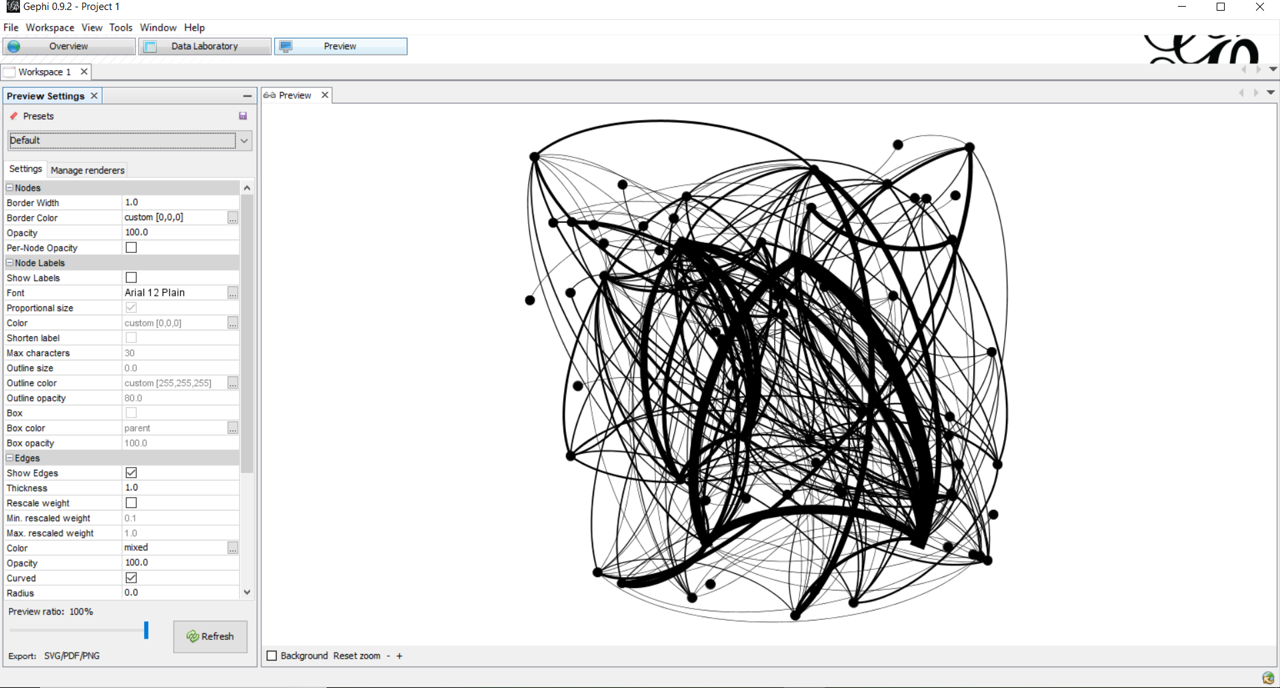
\includegraphics[width=7.5cm]{4.png} }}%
		%\caption{}%
		\label{fig:example}%
	\end{figure}

    	
	
    \section{References}
    \begin{enumerate}
    	\item Bastian, M., Heymann, S., \& Jacomy, M. 2009 Mar 19. Gephi: An Open Source Software for Exploring and Manipulating Networks. International AAAI Conference on Web and Social Media.
    	\item Les Miserables: coappearance weighted network of characters in the novel Les Miserables. D. E. Knuth, The Stanford GraphBase: A Platform for Combinatorial Computing, Addison-Wesley, Reading, MA (1993)
    \end{enumerate}
 

    
\end{document}